\documentclass[journal]{IEEEtran}
\usepackage{amsmath,amssymb,amsfonts}
\usepackage{tabularx}
\usepackage[utf8]{inputenc} % allow utf-8 input
\usepackage[T1]{fontenc}    % use 8-bit T1 fonts
\usepackage{url}            % simple URL typesetting
\usepackage{booktabs}       % professional-quality tables
\usepackage{amsfonts}       % blackboard math symbols
\usepackage{nicefrac}       % compact symbols for 1/2, etc.
\usepackage{microtype}      % microtypography
\usepackage{graphicx}
\usepackage{float}
\restylefloat{table}
\usepackage{hyperref}
\usepackage{multicol}
\usepackage{caption}
\usepackage{subcaption}
\usepackage{amsmath}
\usepackage{algorithm}
\usepackage{algpseudocode}
\usepackage{tikz}
\usetikzlibrary{trees}
\usepackage{listings}

\DeclareMathOperator*{\argmax}{arg\,max}  % in your preamble
\DeclareMathOperator*{\argmin}{arg\,min}  % in your preamble

\usepackage{textcomp}


%\usepackage[retainorgcmds]{IEEEtrantools}
%\usepackage{bibentry}
\usepackage{xcolor,soul,framed} %,caption

\usepackage[noadjust]{cite}
%\usepackage{biblatex}
%\bibliographystyle{plain}

\usepackage[font=small]{caption}

%=== TITLE & AUTHORS ====================================================================
\begin{document}
\bstctlcite{IEEEexample:BSTcontrol}
    \title{test}
\title{Accelerate Reinforcement Learning with Prohibitive Boundaries}

\author{ Zongqiang Pang,Liping Bai ~\IEEEmembership{Member,~IEEE,} \thanks{Nanjing Unversity of Posts and Telecommunications, College of Automation \& College of Artificial Intelligence, Nanjing, Jiangsu,210000 China email:zqpang@njupt.edu.cn}}
% ====================================================================
\maketitle
% === ABSTRACT ====================================================================
% =================================================================================
\begin{abstract}
	Prohibitive Boundary is a common concept for atheletic training. Gymnast, divers, figure skaters would wear harness or a coach would be present to prevent themselves from falling while training for new skills. The same is true for children, as parents caringly provide a helping hand instead of just let them try things out themselves. Reinforcement Learning is an extention of approximate dynamic programming, witch reasons backwards and a lookup table is built in the mean time. With the newly added capacity brought about by deep learning, deep reinforcement learning is proven to be a formitable force when it comes to control. However, there is a clear difference between reinforcement learning and human learning. While out joints can have all kinds of combinatorial movement, we only use a few of those even in the most rigirous circumstances. Also, the way we learn to syncronize out joints is not a exhaustive trial and error process. Immitation learning seek to address this issue by provide a model trajectory, and meta-learning see to address this by provide agents with a sense of physics. In this paper, we mimic the prohibitive boundary method we see in atheletic training to provide agents additional clues about the environment. There are two advantages in this proposed scheme. First, the prohibitive boundary prevent premature termination of an episode, which is of particular importance to environment where failure is costly. Second, the prohibitive boundary method accelerate data collection on states/action pair that matters. We implemented the proposed prohibitibe boundary scheme on various OpenAI Gym environments, and for all the experiments carried out, prohibitive boundary has shown to accelerate training. All the code can be found at: \href{https://github.com/BaiLiping/Prohibitive_Boundary}
\end{abstract}
% === KEYWORDS ====================================================================
% =================================================================================
\begin{IEEEkeywords}
Reinforcement Learning, Assisted Reinforcement Leraning, Reward Engineering
\end{IEEEkeywords}
% For peer review papers, you can put extra information on the cover
% page as needed:
 %\ifCLASSOPTIONpeerreview
 %\begin{center} \bfseries EDICS Category: 3-BBND \end{center}
% \fi
%
% For peerreview papers, this IEEEtran command inserts a page break and
% creates the second title. It will be ignored for other modes.
\IEEEpeerreviewmaketitle


% === I. Paper =============================================================
% =================================================================================
\section{Introduction}
\IEEEPARstart{R}{einforcement} learning is the process of methotically extracting information from experiments to gradually bound the policy distribution, maximizing the expected reward along a path. Trajectory Optimization, on the other hand, tries to capture the dynamics of a system with differential or recurssive equations, and reshape the phase portrait with actions at each step. When the first batch of reasonable RL results were introduced, they were met with coldness. The preface of Bertseka's book Neuro Dynamic Programming provides a good sample on how reinforcement learning is perceived by the control community back in 1996: ...These methods (Reinforcement Learning) were aiming to provide effective suboptimal solutions to complex problems of planning and sequential decision making under uncertainty, that for a long time were thought to be intractable. Our first impression was that the new methods were ambitious, overly optimistic, and lacked firm foundation....Three years later, after a lot of study, analysis, and experimentation, we believe that our initial impressions were largely correct. \cite{Bertsekas1996NeuroDynamicP}

\section{Reinforcement Learning}
Things are certainly different today. Reinforment Learning community routinely generates results that seem untainable to the control community. What has changed is not the theoretical foundation of RL, which is as leaky as it was in 1996, but its computational infrastructure. DeepMind introduced DQN which enjoyed the success in Atari games, yet their success are not easy to reproduce. There are lot of tricks when it comes to training of the network etc.

Before 2010, the predominent tools for function approximation are kernel methods, where feature spaces are used to transform nonlinear functions into linear space such that regression can be performed. Today, the default function approximator are neural networks. Another major change in computation is that of GPU based acceleration. Before the advent of CUDA, GPU programming requires PhD in computer graphics. Today, anyone who is proficient in C/C++ can programme GPU to parallelize their compuation. Software packages such as PyTorch and Tensorflow made this even easier.

\section{Reinforcement Learning for Control}
Control communities use the notation system introduced by Lev Pontryagin. State is denoted $ \mathcal{X}$, Action is denoted $\mathcal{U}$ (the first letter of Russian for "Action"), the dynamics and stocasticity is captured by physical model constraints $x_{t+1}=f(x_t,u_t,e_t)$ where e denote the noise of a system. The objective is usually to minimize the cost funtion $\mathcal{J(.)}$. Reinforcement Learning communities use the notation system introduced by Richard Bellman who studied dynamic programming. State is denoted $\mathcal{S}$, Action is denoted $\mathcal{A}$. The dynamics and stochaticity is captured via transition matrix $\mathcal{P}$ of a Markov Decision Process.The objective of RL is the maximize the reward function $\mathcal{R(.)}$. Yet, if we set the transition matrix to be identical to the noise, then it is clear that the underlying process behind these two notation system are exactly the same. The differences are nothing but style. Since the audience of our paper is the control community, we would cast reinforcement learning in the control notation system.

\subsection{Where to Approximate}
The constraints imposed in the Trajectory Optimization formulation manifest themselves directly in policy $\pi(x)$ and resulting in either a narrow band of trajectories or a single optimal solution. However, adjustments in the reinforecement learning formuation is not the policy per se but its distribution. Eventually, what we hope to acheive via learning is a policy distribution, either through policy gradient method or cost to go method, which would maximize the expected reward of a trajectory.

Reinforcement Learning is not a new subject, control researchers probably know it by the name Approximate Dynamic Programming. Yet the major progress in recent years is the enhanced compuation power which brought about the potential of neuronetworks as a to fruition. Most notably the series of wins reinforcement agents such as AlphaGo, AlphaStar forged against the best human players in the respective disciplines.

Broadly speaking, there are three revenues where neuronetwork based approximation can find its way into optimization as shown in \ref{fig:1}. One is learning a dynamics model from samle; Second is policy gradient based learning; Third is approximation of cost to go functions such as value funtion and Q function. The details of the implementation would be specified in the subsequent sections.

\begin{figure}[H]
    \centering
    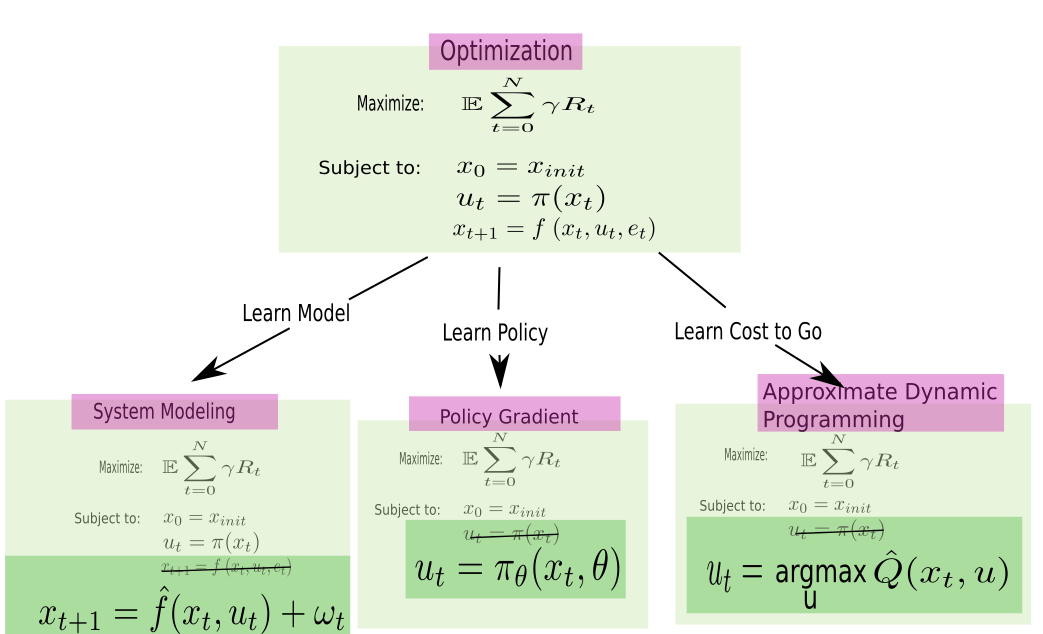
\includegraphics[width=0.5\textwidth]{Control.png}
    \caption{From Optimization to Learning}
    \label{fig:1}
\end{figure}

Before we dive into the detailed researches in each category, we'd like to introduce additional mathematical tools and measurements that has been proven useful in merging reinforcement learning with optimization. One of the most important change of perspectives when control researchers ventures into the land of reinforcement learning is to formulate optimization as an inference problem \cite{Levine2018ReinforcementLA}. Tranditional optimization would translate constraints imposed on the struture into definitive trajectories, subject to disturbance and correction. Yet inference view of optimization is an ever narrowing band od distribution as information trickles in via experiments.

There are two things control researchers should be aware of. One, if you simply apply reinforcement learning as it is written in Richard Sutton's book, it probably won't work for you. Additional statistical learning techniques are required. Two, Statistical learning is booming with ideas at this point. Every newly invented measurement and methods could be pretzeled into a self-sustainly structure if you know how to make such arguments, that does not mean it would be a useful tool for your research.

Here we point out two concepts: Mutual Information and Baysian NeuroNet, which have proven to be integral for converting optimization into an inference.

The go to text book for reinforcement learning community is that of Richard Sutton \cite{Sutton1998IntroductionTR}. In the system contstructed by Richard, the objective of an agent is to maximize discounted reward. This formulation is proven a sound goal in the context of video games. However, for optimizations with a physics underpining, reward maximization is not adequate for noise and disturbances.

Exploration and Exploitation trade off is something studied exhaustively in the reinforcement learning community. A common strategy is $\epsilon$ greedy policy where the value of epsilon decays as the learning progresses. Yet, the decaying rate is a hyperparater that need to be tuned. Is there are more sysmtmatical way to balance the exploration and exploitation trade-off? This is particularly important for control related training since this application has considerable amount of disturbance and noise. If the policy converges too soon, any subsequent disturce can deviate the trajectory to the extend that it is no longer controllable.

The intuition behind maximum entropy reinforcenement learning is the heuristic that when we don't know all the circumstance, we should prioritize options that could give us more choices regardless of how the system dynamics turns out to be. Statitically speaking, this means we should maximize the entropy of a distribution, which measures how uncertain or how broad the distributionb is.

The mathematical measurement used is mutual information \cite{Kullback1951ONIA}. It measures how much information regarding the random variable X is contained in the distribution of random variable Y. A reasonable question to ask is that out of all those measurements which captures "distance" in meansurement theory, why a divergence is chosen? Turns out, this choice is made because of its computational convenience, much like exponentials are chosen in integral transform because its nice features.

\subsection{Intuition Behind Neural Network}
By now, neural network is widely accepted that as the universal function approximator \cite{Hornik1991ApproximationCO} and the grandfathers of this field such as Andrew Ng and Geoffrey Hinton are also its most proficient proselytizer. Yet not that many materials goes into the intution behind neural network. Here we provide control researchers with minimal exposure to deep learning the graphical reasonings behind neural network. For people who are interested in tracing the deveopment of this subject, we list the following seminal papers: \cite{Schwartz1989TheNC} \cite{Hornik1989MultilayerFN}........


\section{Prohibitive Boundary}
Have you ever wondered how do world class athelets such as gymnists, figure skaters, divers accomplish feats that are seemingly impossible to us ordinary human?  While bruises, torn ligaments, broken bones, even concausion are part of being an athelete, those injuries are by no means trivial and should be minimized at any cost. Should athletes train the same way as reinforcement learning agents, they would be dead before they can pick up any skill.Prohibitive Boundaries, implemented with either human coach or training harnesses is integral part of atheletic skills acquisition, as examplified by the following figures:

\begin{figure}[H]
\centering
\begin{subfigure}{0.25\textwidth}
  \centering
  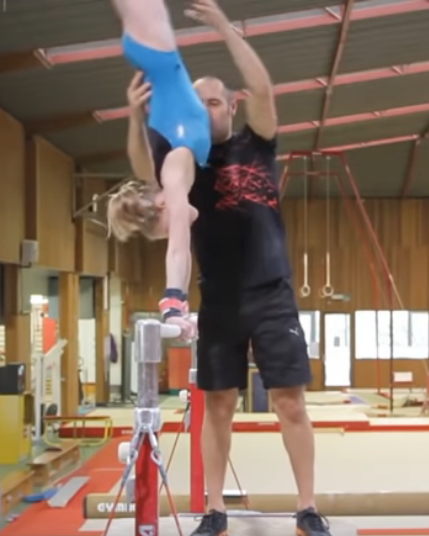
\includegraphics[width=\linewidth]{/img/training1.png}
  \caption{Human Prohibitive Boundary}
\end{subfigure}%
\begin{subfigure}{.25\textwidth}
  \centering
  \includegraphics[width=\linewidth]{/img/traning2.png}
  \caption{Harness Prohibitive Boundary}
\end{subfigure}
\caption{Prohibitive Boundary in Atheletic Training}
\label{fig:athelet}
\end{figure}

\href{https://www.youtube.com/playlist?list=PLyqL4-20ZuTRo-DysDQBGDnwZsrySXP4b}{How Athletes Utilize Prohibitive Boundary During Their Training}


Do they train as it would we train the agents in a reinforcement learning setup? The answer is clearly now, since for those athlets, failure means catestrophic consequences such as broken bones, torn ligaments, concausion etc. While being atheletes means accepting the possibility of permenent harm from training, the entire sport industry try hard to minimize the downside of training.


\subsection{Experiments on OpenAI Gym}
\subsubsection{CartPole}
\subsubsection{Inverted Pendulum}
\subsubsection{Inverted Double Pendulum}
\subsubsection{Mountain Car}
\subsubsection{}


\section{Conclution}




\bibliographystyle{IEEEtran}
\bibliography{Bibliography}
%\printbibliography



\end{document}
